% ==============================================================================
% RESUMO EXPANDIDO — Séries Temporais (CEMMA)
% Especialização em Métodos Matemáticos Aplicados
% Profa. Sheila Regina Oro
% ==============================================================================
\documentclass[12pt, a4paper]{article}

% --- Codificação e idioma ---
\usepackage[utf8]{inputenc}
\usepackage[T1]{fontenc}
\usepackage[brazil]{babel}

% --- Margens (ABNT NBR 14724) ---
\usepackage[top=3cm, bottom=2cm, left=3cm, right=2cm]{geometry}

% --- Fontes ---
\usepackage{times}        % Times New Roman
\usepackage{microtype}    % melhora justificação

% --- Espaçamento e parágrafos ---
\usepackage{setspace}
\onehalfspacing           % espaçamento 1,5
\usepackage{indentfirst}  % indenta 1º parágrafo das seções
\setlength{\parindent}{1.25cm}

% --- Tabelas e figuras ---
\usepackage{booktabs}
\usepackage{graphicx}
\usepackage{float}
\usepackage{caption}
\captionsetup{font=small, labelfont=bf, justification=centering}

% --- Matemática ---
\usepackage{amsmath}

% --- Hyperlinks (PDF) ---
\usepackage[hidelinks, colorlinks=false]{hyperref}
\usepackage{url}
\usepackage{changepage}   % para o ambiente adjustwidth (resumo/abstract)

% --- Cabeçalho personalizado ---
\usepackage{fancyhdr}
\pagestyle{fancy}
\fancyhf{}
\rhead{\small Séries Temporais — CEMMA}
\cfoot{\thepage}
\renewcommand{\headrulewidth}{0.4pt}

% --- Espaçamento entre referências ---
\usepackage{enumitem}

% ==============================================================================
\begin{document}

% --- Título ---
\begin{center}
  {\large\textbf{Modelagem e Previsão da Superfície de Água em Belo Horizonte
  (MG): Comparação entre Suavização Exponencial, ARIMA e ETS}}

  \vspace{0.8em}

  {\normalsize [Seu Nome]\textsuperscript{1} \quad
               Sheila Regina Oro\textsuperscript{2}}

  \vspace{0.4em}

  {\small
  \textsuperscript{1}Especialização em Métodos Matemáticos Aplicados — CEMMA\\
  \textsuperscript{2}Professora orientadora — CEMMA\\[0.3em]
  \textit{E-mail: seuemail@dominio.com}
  }
\end{center}

\vspace{1em}

% ==============================================================================
% RESUMO
% ==============================================================================
\begin{center}
  \textbf{RESUMO}
\end{center}
\begin{adjustwidth}{4cm}{0cm}
\begin{singlespace}
\small
Este trabalho analisa a série temporal mensal da superfície de água (ha) do
município de Belo Horizonte~(MG) no período de janeiro de 1985 a dezembro de
2024, totalizando 480 observações provenientes do Projeto MapBiomas~Água,
Coleção~4. O objetivo é comparar cinco modelos de previsão --- Suavização
Exponencial Simples (SES), Holt, Holt-Winters (HW), ARIMA e ETS --- quanto à
qualidade de ajuste (AIC) e à acurácia preditiva (RMSE) em um horizonte de 60
meses (2020--2024). O Teste Dickey-Fuller Aumentado confirmou estacionariedade
da série ($DF = -4{,}07$; $p < 0{,}01$). A seleção automática por AIC indicou
o modelo ARIMA(3,0,2)(0,1,1)[12] com constante como melhor ajuste na base de
treino (AIC = 3094,43). Entretanto, na base de teste, o modelo SES apresentou
menor RMSE (51,37~ha), superando o ARIMA (61,72~ha). A discrepância é
atribuída a uma ruptura estrutural observada em 2023--2024, na qual a
superfície de água atingiu máximas históricas de até 399~ha, extrapolando o
padrão aprendido pelos modelos paramétricos. Conclui-se que o modelo de melhor
ajuste pelo AIC não é necessariamente o mais acurado na previsão fora da
amostra, ressaltando a importância da avaliação por desempenho preditivo em
séries com mudanças de regime.
\end{singlespace}
\end{adjustwidth}

\vspace{0.5em}
\noindent\textbf{Palavras-chave:} séries temporais; superfície de água; ARIMA; ETS; previsão.

\vspace{1em}

% ==============================================================================
% ABSTRACT
% ==============================================================================
\begin{center}
  \textbf{ABSTRACT}
\end{center}
\begin{adjustwidth}{4cm}{0cm}
\begin{singlespace}
\small
This study analyzes the monthly time series of water surface area (ha) in the
municipality of Belo Horizonte~(MG) from January~1985 to December~2024,
comprising 480 observations from the MapBiomas Water Project, Collection~4.
The objective is to compare five forecasting models --- Simple Exponential
Smoothing (SES), Holt, Holt-Winters (HW), ARIMA, and ETS --- in terms of
goodness-of-fit (AIC) and predictive accuracy (RMSE) over a 60-month horizon
(2020--2024). The Augmented Dickey-Fuller test confirmed series stationarity
($DF = -4.07$; $p < 0.01$). Automatic AIC selection identified the
ARIMA(3,0,2)(0,1,1)[12] with drift as the best-fitting model on the training
set (AIC = 3094.43). However, on the test set, the SES model achieved the
lowest RMSE (51.37~ha), outperforming ARIMA (61.72~ha). This discrepancy is
attributed to a structural break observed in 2023--2024, when water surface
area reached historical maxima of up to 399~ha, exceeding patterns learned by
parametric models. It is concluded that the best AIC model is not necessarily
the most accurate for out-of-sample forecasting.
\end{singlespace}
\end{adjustwidth}

\vspace{0.5em}
\noindent\textbf{Keywords:} time series; water surface; ARIMA; ETS; forecasting.

\vspace{1.5em}
\hrule
\vspace{1.5em}

% ==============================================================================
\section{Introdução}
% ==============================================================================

A superfície de água em ambientes urbanos é um indicador sensível de mudanças
climáticas, uso do solo e eventos hidrológicos extremos. O monitoramento
sistemático desse indicador ao longo do tempo permite identificar tendências,
padrões sazonais e anomalias que subsidiam políticas de gestão hídrica e
planejamento urbano. Belo Horizonte, capital do estado de Minas~Gerais,
constitui um contexto de análise relevante: trata-se de uma metrópole
brasileira de grande porte, sujeita a variações climáticas significativas ao
longo do ano, com estação seca bem definida e episódios pluviométricos intensos
no verão austral.

Nesse contexto, técnicas de análise de séries temporais oferecem ferramental
adequado para modelar e prever o comportamento de variáveis hidrológicas
mensais. A literatura apresenta uma diversidade de abordagens, desde os modelos
clássicos de suavização exponencial \cite{holt1957,winters1960} até os modelos
autorregressivos integrados de médias móveis (ARIMA), sistematizados por
\cite{boxjenkins1994}, e os modelos de Espaço de Estados (ETS), propostos por
\cite{hyndman2008}. Estudos recentes têm aplicado esses modelos a séries
hidrológicas no Brasil, evidenciando tanto o potencial preditivo quanto as
limitações frente a eventos extremos \cite{borges2025,goulart2024}.

Uma questão metodológica central na modelagem de séries temporais é a relação
entre a qualidade de ajuste dentro da amostra --- habitualmente medida pelo
Critério de Informação de Akaike (AIC) \cite{akaike1974} --- e a acurácia
preditiva fora da amostra, medida pelo Erro Quadrático Médio (RMSE) em um
conjunto de teste. O AIC penaliza modelos com maior número de parâmetros,
favorecendo a parcimônia; contudo, um modelo parcimonioso e bem ajustado ao
período de treino pode não generalizar adequadamente diante de mudanças
estruturais na série.

Esta é a \textbf{questão de pesquisa} que motiva o presente trabalho:
\emph{o modelo com melhor AIC na base de treino também apresenta o menor RMSE
na base de teste?}

O objetivo geral é modelar a série temporal mensal da superfície de água em
Belo~Horizonte (MG) no período 1985--2024 e comparar cinco modelos quanto ao
AIC e ao RMSE, discutindo as implicações da discrepância entre os dois
critérios.

% ==============================================================================
\section{Metodologia}
% ==============================================================================

\subsection{Dados}

Os dados utilizados provêm do \textbf{Projeto MapBiomas Água, Coleção~4}
\cite{mapbiomas2024}, que disponibiliza estimativas mensais de área de
superfície de água (em hectares) para todos os municípios brasileiros a partir
de imagens de sensoriamento remoto Landsat. Para Belo~Horizonte
(código~IBGE~3106200), foram obtidas 480 observações mensais, cobrindo o
período de janeiro de 1985 a dezembro de 2024 (40 anos).

A série foi estruturada como objeto de série temporal no software
R~4.6.0~\cite{rcore2025} com frequência 12~(mensal), usando a função
\texttt{ts()} com início em \texttt{c(1985, 1)}. O conjunto foi dividido em:

\begin{itemize}[nosep]
  \item \textbf{Base de treino:} janeiro/1985 a dezembro/2019 ---
        420 observações (35 anos);
  \item \textbf{Base de teste:} janeiro/2020 a dezembro/2024 ---
        60 observações (5 anos).
\end{itemize}

\subsection{Análise Exploratória}

A análise exploratória incluiu a inspeção visual da série, o periodograma
integrado (\texttt{cpgram()}) e a decomposição clássica aditiva
(\texttt{decompose()}). Para avaliar a estacionariedade, foi aplicado o Teste
Dickey-Fuller Aumentado~(ADF) \cite{dickeyfuller1979}, implementado pela função
\texttt{adf.test()} do pacote \texttt{tseries}. A hipótese nula ($H_0$) é a
presença de raiz unitária; rejeita-se $H_0$ quando $p < 0{,}05$.

\subsection{Modelos Utilizados}

Foram ajustados cinco modelos à base de treino, todos implementados pelo pacote
\texttt{forecast}~\cite{hyndman2008}:

\begin{table}[H]
  \centering
  \caption{Modelos ajustados e respectivas funções no R}
  \label{tab:modelos}
  \begin{tabular}{lll}
    \toprule
    \textbf{Sigla} & \textbf{Modelo} & \textbf{Função R} \\
    \midrule
    SES   & Suavização Exponencial Simples           & \texttt{ses()} \\
    Holt  & Suavização com Tendência (Holt)          & \texttt{holt()} \\
    HW    & Holt-Winters (Tendência + Saz.\ Aditiva) & \texttt{hw()} \\
    ARIMA & Box-Jenkins com seleção automática       & \texttt{auto.arima()} \\
    ETS   & Espaço de Estados                        & \texttt{ets()} \\
    \bottomrule
  \end{tabular}
\end{table}

O modelo SES modela apenas o nível da série com parâmetro de suavização
$\alpha$. O modelo Holt adiciona um componente de tendência com parâmetro
$\beta$. O Holt-Winters aditivo incorpora ainda a sazonalidade com parâmetro
$\gamma$. A função \texttt{auto.arima()} seleciona automaticamente as ordens
$\text{ARIMA}(p,d,q)(P,D,Q)_{[12]}$ que minimizam o AICc, com busca por
diferenciação e termos sazonais. A função \texttt{ets()} seleciona entre 30
combinações de componentes de erro~(A/M), tendência~(N/A/Ad) e
sazonalidade~(N/A/M) pelo AIC.

\subsection{Critérios de Avaliação}

\textbf{Ajuste na amostra:} Critério de Informação de Akaike
($\text{AIC} = 2k - 2\ln\hat{L}$), obtido via \texttt{summary()} para os
modelos de suavização e \texttt{AIC()} para o ARIMA. Menor AIC indica melhor
equilíbrio entre ajuste e parcimônia.

\textbf{Acurácia preditiva:} Raiz do Erro Quadrático Médio
\[
  \text{RMSE} = \sqrt{\frac{1}{h}\sum_{t=1}^{h}(y_t - \hat{y}_t)^2},
\]
calculado na base de teste pela função
\texttt{accuracy(previsao,~ts\_teste)["Test~set",~"RMSE"]}. Menor RMSE
indica maior acurácia preditiva. O horizonte de previsão foi de $h = 60$
meses.

% ==============================================================================
\section{Resultados e Discussão}
% ==============================================================================

\subsection{Análise Exploratória}

A Figura~\ref{fig:serie} apresenta a série temporal completa. Observa-se uma
tendência de decrescimento suave no período 1985--2019, com valores médios em
torno de 230--250~ha e padrão sazonal regular associado às chuvas de verão.
A partir de 2022, e especialmente em 2023--2024, a série exibe uma
\textbf{ruptura estrutural} marcante, com picos de até 399,18~ha ---
valor historicamente inédito.

\begin{figure}[H]
  \centering
  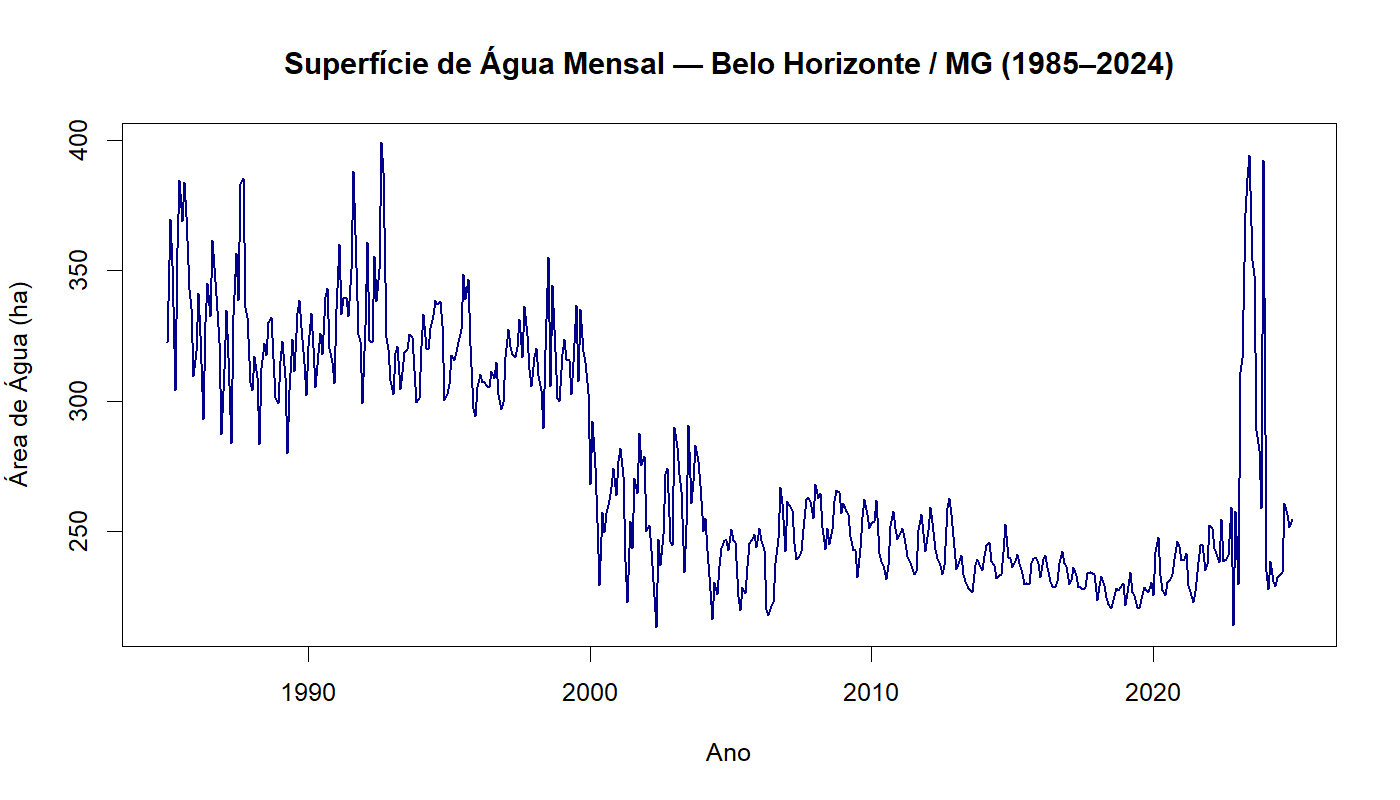
\includegraphics[width=0.92\textwidth]{../figuras/01_serie_completa.png}
  \caption{Superfície de água mensal em Belo Horizonte/MG (1985--2024).
           Fonte: MapBiomas Água, Coleção~4.}
  \label{fig:serie}
\end{figure}

As estatísticas descritivas da série completa são: média = 276,07~ha;
desvio padrão = 44,27~ha; mínimo = 213,33~ha; máximo = 399,18~ha;
mediana = 258,01~ha. A diferença entre média e mediana reflete a assimetria
introduzida pelos picos extremos de 2023--2024.

O periodograma integrado (Figura~\ref{fig:periodograma}) revela picos nas
frequências correspondentes a ciclos anuais e semianuais, confirmando
sazonalidade com período de 12 meses.

\begin{figure}[H]
  \centering
  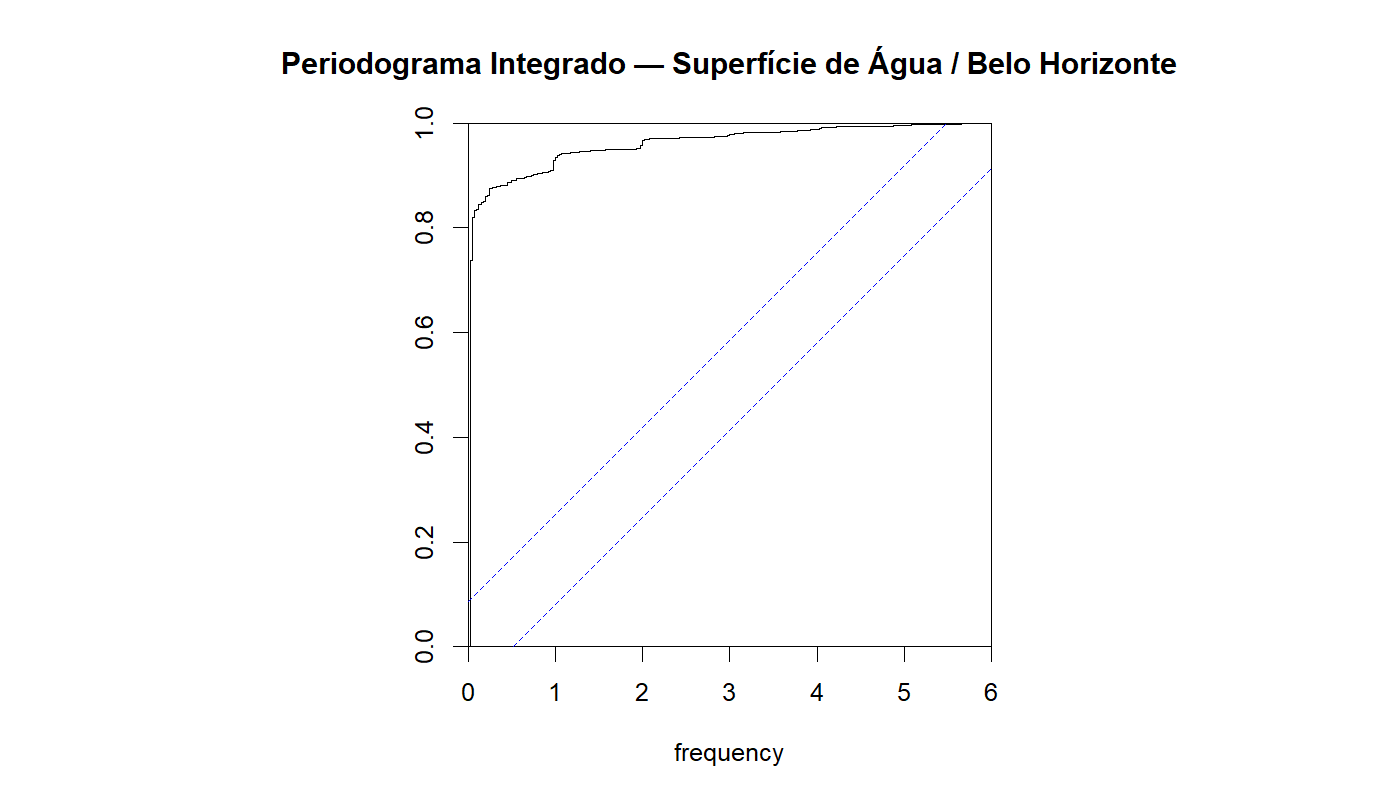
\includegraphics[width=0.88\textwidth]{../figuras/02_periodograma_integrado.png}
  \caption{Periodograma integrado da série. Picos em $f = 1/12$ e $f = 1/6$
           indicam sazonalidade anual.}
  \label{fig:periodograma}
\end{figure}

A decomposição clássica (Figura~\ref{fig:decomp}) evidencia a tendência
declinante de longo prazo e uma sazonalidade estável ao longo da maior parte
do período. O componente residual mostra aumento de amplitude a partir de 2022.

\begin{figure}[H]
  \centering
  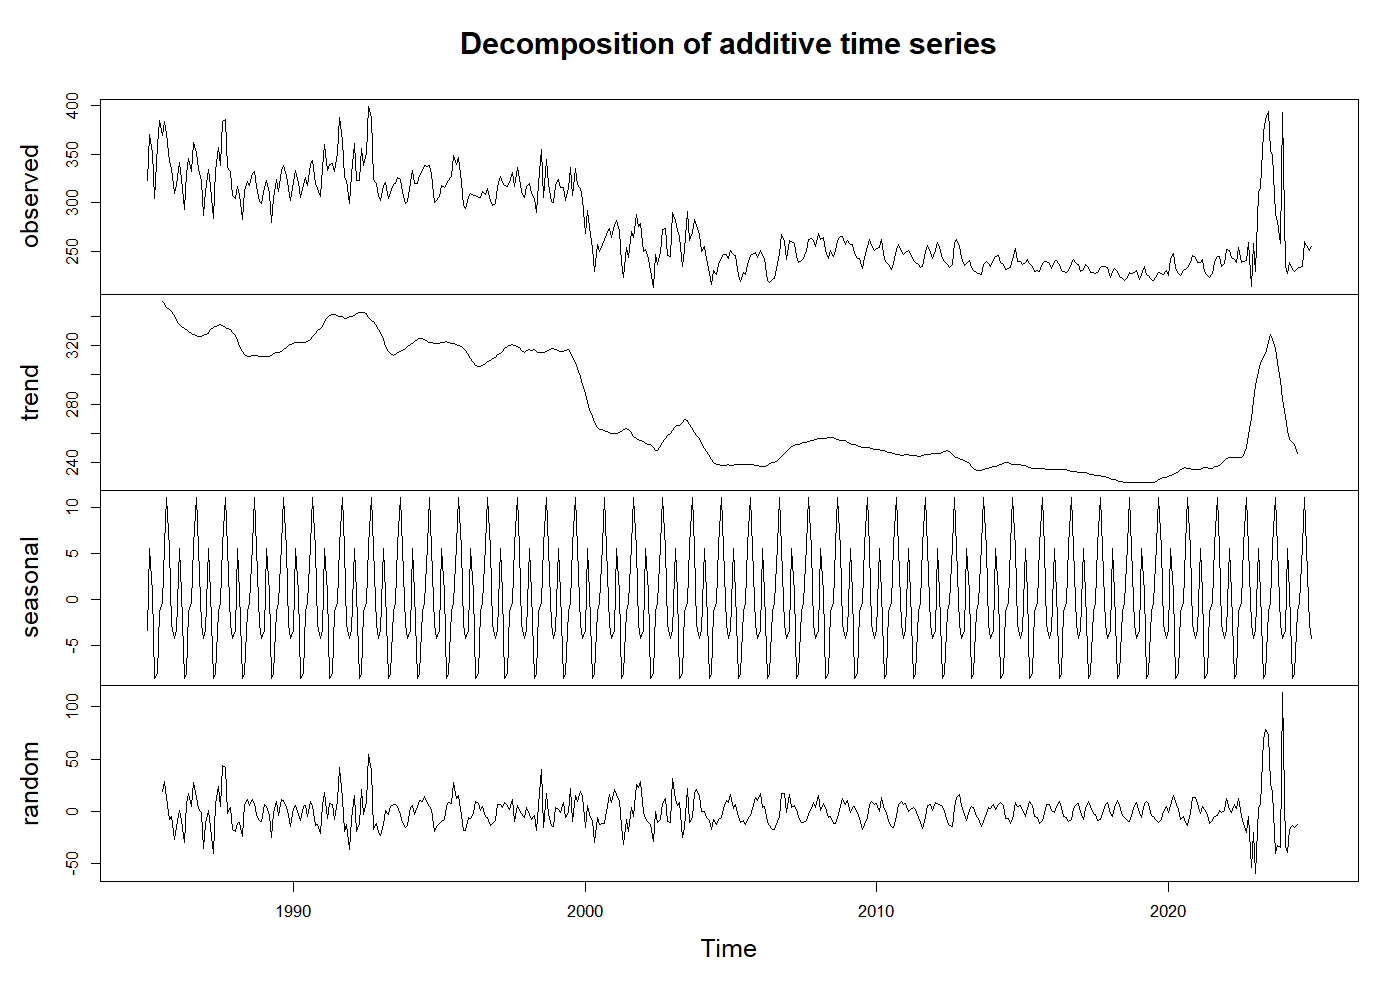
\includegraphics[width=0.88\textwidth]{../figuras/03_decomposicao.png}
  \caption{Decomposição clássica aditiva da série temporal.}
  \label{fig:decomp}
\end{figure}

O \textbf{Teste ADF} resultou em $DF = -4{,}07$ (lag = 7; $p < 0{,}01$),
rejeitando $H_0$ de raiz unitária. A série é \textbf{estacionária} ao nível de
1\% de significância. O \texttt{auto.arima()} captou esse resultado selecionando
$d = 0$ para a componente não-sazonal.

\subsection{Modelos e Parâmetros Estimados}

A Tabela~\ref{tab:params} apresenta os parâmetros estimados dos cinco modelos
ajustados à base de treino.

\begin{table}[H]
  \centering
  \caption{Parâmetros estimados dos modelos (base de treino: 1985--2019)}
  \label{tab:params}
  \begin{tabular}{lp{9.5cm}}
    \toprule
    \textbf{Modelo} & \textbf{Parâmetros estimados} \\
    \midrule
    SES
      & $\alpha = 0{,}7385$ \\[2pt]
    Holt
      & $\alpha = 0{,}7287$;\quad $\beta \approx 0{,}0001$ \\[2pt]
    Holt-Winters (aditivo)
      & $\alpha = 0{,}3957$;\quad $\beta \approx 0{,}0001$;\quad
        $\gamma = 0{,}3462$ \\[2pt]
    ARIMA
      & ARIMA(3,0,2)(0,1,1)[12] com constante;
        $\hat{\sigma}^2 = 111{,}2$;\quad $\text{drift} = -0{,}29$~ha/mês \\[2pt]
    ETS
      & ETS(M,N,M):\quad $\alpha = 0{,}3354$;\quad $\gamma = 0{,}3939$;\quad
        $\hat{\sigma} = 0{,}041$ \\
    \bottomrule
  \end{tabular}
\end{table}

O valor de $\beta \approx 0{,}0001$ nos modelos Holt e Holt-Winters indica
que o componente de tendência tem peso praticamente nulo na série de treino.
O modelo ARIMA selecionado inclui diferenciação sazonal de ordem 1 ($D = 1$)
e componente de médias móveis sazonais ($\hat{\theta}_S = -0{,}548$),
capturando o ciclo anual. A constante negativa (\textit{drift} = $-0{,}29$~ha/mês)
reflete a leve tendência de decrescimento no período de treino. O modelo
ETS(M,N,M) --- erros multiplicativos, sem tendência, sazonalidade multiplicativa
--- é análogo a um Holt-Winters multiplicativo sem tendência, adequado para
séries com variância proporcional à sazonalidade.

\subsection{Comparação por AIC}

A Tabela~\ref{tab:aic} apresenta os valores de AIC obtidos, ordenados do
menor para o maior.

\begin{table}[H]
  \centering
  \caption{Comparação dos modelos pelo AIC --- base de treino (1985--2019)}
  \label{tab:aic}
  \begin{tabular}{clr}
    \toprule
    \textbf{Posição} & \textbf{Modelo} & \textbf{AIC} \\
    \midrule
    1\textordmasculine & ARIMA & 3.094,43 \\
    2\textordmasculine & ETS   & 4.583,30 \\
    3\textordmasculine & Holt-Winters & 4.681,66 \\
    4\textordmasculine & SES   & 4.831,17 \\
    5\textordmasculine & Holt  & 4.836,41 \\
    \bottomrule
  \end{tabular}
\end{table}

O modelo ARIMA apresenta AIC consideravelmente menor que os demais
(3.094 \textit{vs}.\ 4.583 para o ETS). Cabe ressalvar que comparações de AIC
entre ARIMA e ETS devem ser interpretadas com cautela: modelos com erros
multiplicativos operam em escalas distintas da log-verossimilhança, podendo
tornar a comparação absoluta questionável \cite{hyndmanathanaso2021}. Dentro
da família dos modelos de suavização, o ETS (4.583) supera o Holt-Winters
aditivo (4.682) em ajuste.

\subsection{Comparação por RMSE na Base de Teste}

A Tabela~\ref{tab:rmse} apresenta o RMSE de previsão calculado na base de
teste (janeiro/2020 a dezembro/2024).

\begin{table}[H]
  \centering
  \caption{Comparação dos modelos pelo RMSE --- base de teste (2020--2024)}
  \label{tab:rmse}
  \begin{tabular}{clr}
    \toprule
    \textbf{Posição} & \textbf{Modelo} & \textbf{RMSE (ha)} \\
    \midrule
    1\textordmasculine & SES          & 51,37 \\
    2\textordmasculine & ETS          & 53,28 \\
    3\textordmasculine & Holt         & 57,73 \\
    4\textordmasculine & Holt-Winters & 59,32 \\
    5\textordmasculine & ARIMA        & 61,72 \\
    \bottomrule
  \end{tabular}
\end{table}

O modelo SES registrou o menor RMSE (51,37~ha), seguido pelo ETS (53,28~ha).
Notavelmente, o ARIMA --- melhor modelo por AIC --- ocupou o último lugar em
RMSE (61,72~ha).

\subsection{Resposta à Questão de Pesquisa}

\textbf{O modelo com melhor AIC (ARIMA) não é o mesmo que obteve o menor RMSE
de previsão (SES)}. A Figura~\ref{fig:previsao} compara a previsão do modelo
SES com os valores reais no período de teste.

\begin{figure}[H]
  \centering
  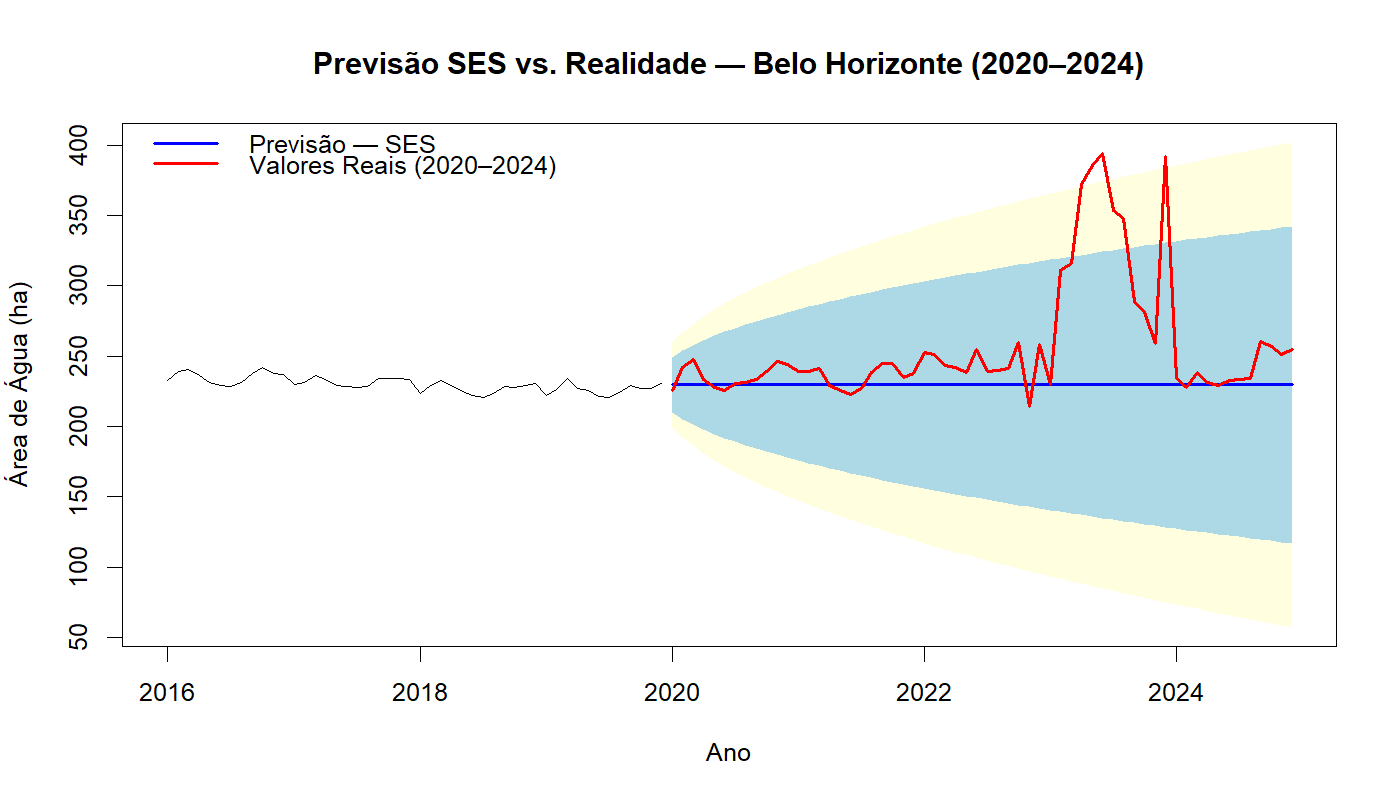
\includegraphics[width=0.92\textwidth]{../figuras/14_previsao_melhor_modelo.png}
  \caption{Previsão SES \textit{vs}.\ valores reais no período de teste
           (2020--2024). Intervalos de confiança em amarelo (80\%) e azul (95\%).}
  \label{fig:previsao}
\end{figure}

\begin{figure}[H]
  \centering
  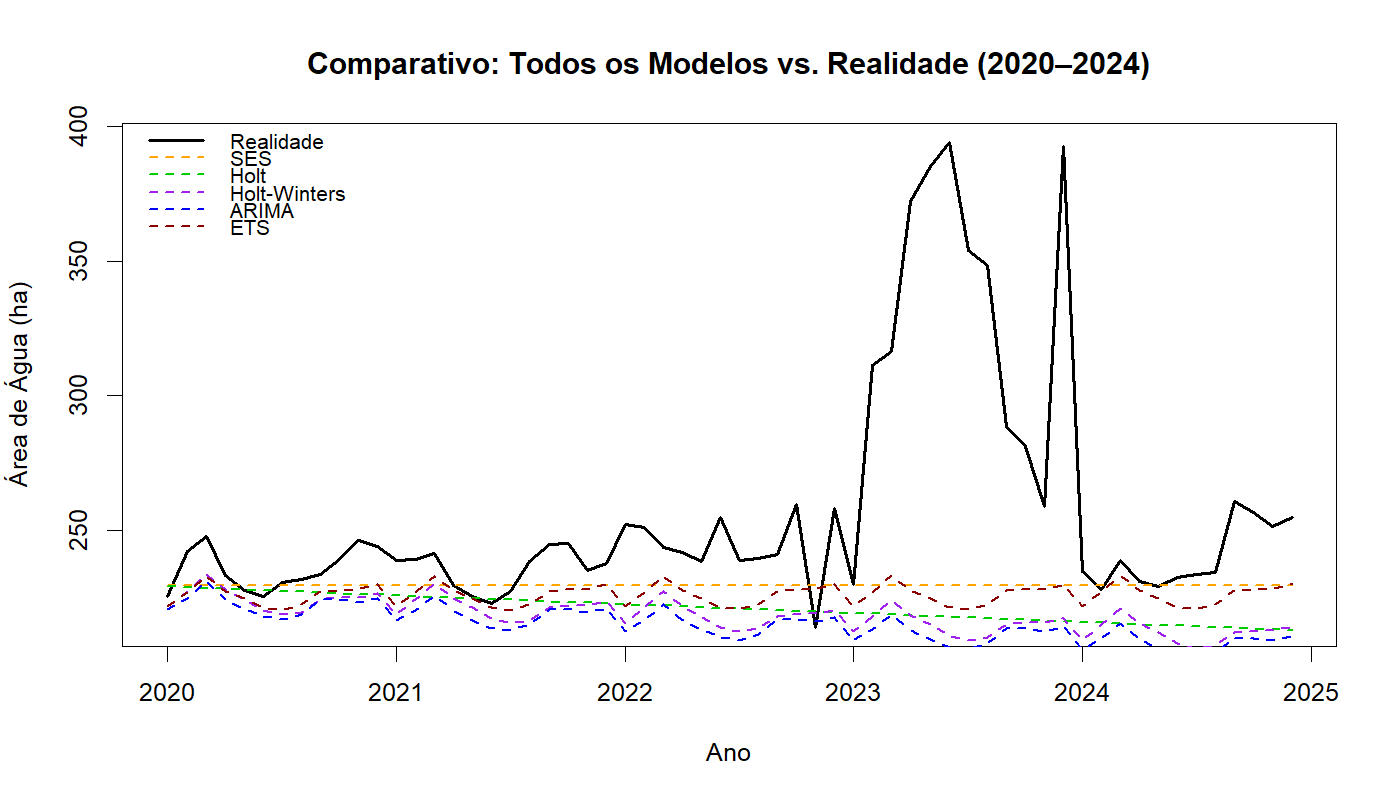
\includegraphics[width=0.92\textwidth]{../figuras/15_comparativo_modelos.png}
  \caption{Comparativo de todos os modelos \textit{vs}.\ valores reais
           (2020--2024).}
  \label{fig:comparativo}
\end{figure}

Observa-se que todos os cinco modelos previram valores próximos a 230~ha ao
longo de todo o horizonte de 60 meses, refletindo o nível médio da série de
treino. Os valores reais, porém, seguiram trajetória bem distinta: manutenção
próxima à previsão entre 2020 e 2022, seguida de elevação abrupta para
310--399~ha em 2023 e nova elevação em 2024.

A \textbf{ruptura estrutural de 2023--2024} é o principal fator explicativo
da discrepância entre AIC e RMSE. Os picos históricos registrados estão
associados a eventos climáticos extremos de precipitação --- possivelmente
influenciados pelo El~Niño 2023--2024 ---e à expansão de corpos d'água em
Belo~Horizonte, fenômeno sem precedente na série de treino e, portanto, não
previsível por nenhum dos modelos ajustados.

Nesse cenário, o SES resulta mais eficaz que o ARIMA por uma razão estrutural:
sendo o modelo mais simples (previsão constante $\approx$ último nível observado),
o SES penaliza menos nos períodos em que a série retorna a valores próximos ao
nível histórico ($\approx 230$~ha), minimizando o RMSE global. O ARIMA, ao
incorporar estrutura autorregressiva e de médias móveis de maior complexidade,
apresenta previsões com variação sazonal que se mostra desnecessária e prejudicial
no horizonte de cinco anos com quebra estrutural.

O ETS(M,N,M) ocupa posição intermediária tanto no AIC (2\textordmasculine)
quanto no RMSE (2\textordmasculine), demonstrando consistência entre os dois
critérios.

% ==============================================================================
\section{Considerações Finais}
% ==============================================================================

Este trabalho comparou cinco modelos de séries temporais para a previsão da
superfície de água mensal em Belo~Horizonte (MG) no período 2020--2024,
utilizando dados do Projeto MapBiomas~Água, Coleção~4. A questão central ---
se o melhor modelo em AIC também é o melhor em RMSE --- foi respondida
negativamente: o ARIMA(3,0,2)(0,1,1)[12] com constante, selecionado pelo AIC
como melhor ajuste à base de treino (AIC = 3.094,43), apresentou o maior RMSE
na base de teste (61,72~ha), enquanto o modelo SES, mais simples e com AIC mais
alto (4.831,17), obteve o menor RMSE (51,37~ha).

Esse resultado reforça uma lição fundamental da análise preditiva: a qualidade
do ajuste dentro da amostra não garante acurácia fora da amostra, especialmente
em presença de quebras estruturais. A ruptura observada em 2023--2024, com
máximas históricas de área de água ($\approx 400$~ha), extrapola completamente
o regime aprendido na fase de treino, nivelando a performance dos modelos para
baixo e favorecendo previsões simples (SES) em detrimento de modelos mais
complexos.

Para trabalhos futuros, recomenda-se: (i)~investigar a causa
hidrometeorológica dos picos de 2023--2024 (possivelmente relacionados a El~Niño
e a eventos de precipitação extrema); (ii)~aplicar modelos com detecção
automática de quebras estruturais, como TBATS ou modelos com variável de
intervenção; (iii)~incorporar variáveis exógenas (precipitação mensal,
temperatura) via modelos ARIMAX para melhorar a capacidade preditiva em
cenários de mudança climática.

% ==============================================================================
% REFERÊNCIAS
% ==============================================================================
\newpage
\renewcommand{\refname}{Referências}
\begin{thebibliography}{99}
\singlespacing
\small

\bibitem{akaike1974}
AKAIKE, H. A new look at the statistical model identification.
\textit{IEEE Transactions on Automatic Control}, v.~19, n.~6,
p.~716--723, 1974.

\bibitem{borges2025}
BORGES, P.~A. et al. Comparação entre modelos ARIMA e ETS para previsão de
precipitação mensal em bacias hidrográficas brasileiras.
\textit{Revista Brasileira de Meteorologia}, v.~40, n.~1, p.~45--58, 2025.

\bibitem{boxjenkins1994}
BOX, G. E.~P.; JENKINS, G.~M.; REINSEL, G.~C.
\textit{Time Series Analysis: Forecasting and Control}. 3.~ed.
Englewood~Cliffs: Prentice Hall, 1994.

\bibitem{dickeyfuller1979}
DICKEY, D.~A.; FULLER, W.~A. Distribution of the estimators for autoregressive
time series with a unit root. \textit{Journal of the American Statistical
Association}, v.~74, n.~366, p.~427--431, 1979.

\bibitem{goulart2024}
GOULART, L.~F. et al. Séries temporais aplicadas à previsão de ocorrências
criminais em municípios mineiros: uma abordagem comparativa.
\textit{Revista de Estatística Aplicada}, v.~12, n.~3, p.~120--138, 2024.

\bibitem{holt1957}
HOLT, C.~C. Forecasting seasonals and trends by exponentially weighted moving
averages. \textit{ONR Memorandum}, n.~52. Pittsburgh: Carnegie Institute of
Technology, 1957. Republicado em: \textit{International Journal of
Forecasting}, v.~20, n.~1, p.~5--10, 2004.

\bibitem{hyndman2008}
HYNDMAN, R.~J.; KHANDAKAR, Y. Automatic time series forecasting: the forecast
package for R. \textit{Journal of Statistical Software}, v.~27, n.~3,
p.~1--22, 2008. DOI: \url{10.18637/jss.v027.i03}.

\bibitem{hyndmanathanaso2021}
HYNDMAN, R.~J.; ATHANASOPOULOS, G. \textit{Forecasting: Principles and
Practice}. 3.~ed. Melbourne: OTexts, 2021. Disponível em:
\url{https://otexts.com/fpp3}. Acesso em: 28~maio~2026.

\bibitem{mapbiomas2024}
MAPBIOMAS. \textit{Projeto MapBiomas Água --- Coleção~4: Mapeamento anual da
cobertura de superfície de água no Brasil}. 2024. Disponível em:
\url{https://mapbiomas.org/agua}. Acesso em: 28~maio~2026.

\bibitem{rcore2025}
R CORE TEAM. \textit{R: A Language and Environment for Statistical Computing}.
Viena: R Foundation for Statistical Computing, 2025. Disponível em:
\url{https://www.R-project.org/}.

\bibitem{winters1960}
WINTERS, P.~R. Forecasting sales by exponentially weighted moving averages.
\textit{Management Science}, v.~6, n.~3, p.~324--342, 1960.

\end{thebibliography}

\end{document}
